\documentclass{standalone}
\usepackage{tikz}
\usetikzlibrary{automata, positioning, arrows.meta}

\begin{document}
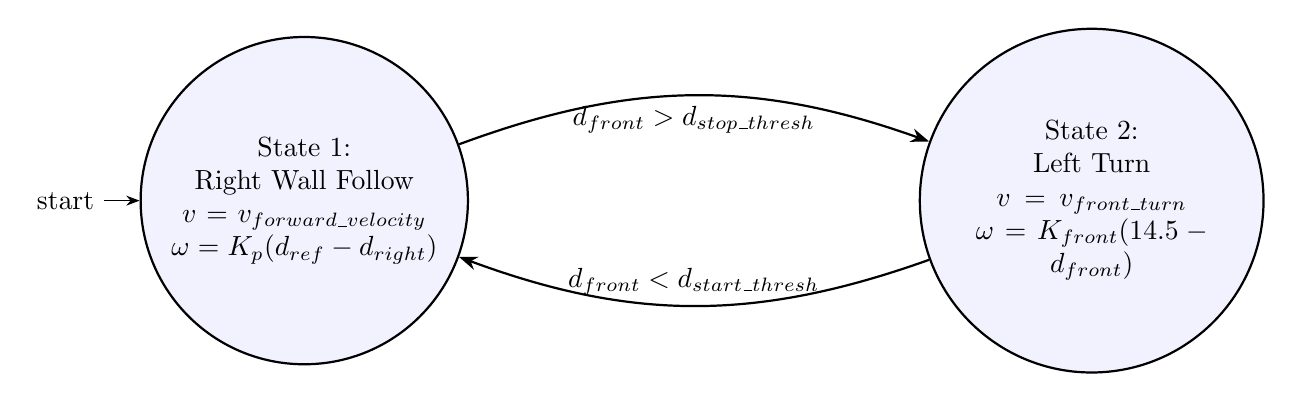
\begin{tikzpicture}[>=Stealth, node distance=6cm, on grid, auto, every state/.style={thick, fill=blue!5, text width=3.5cm, align=center}]

    \node[state, initial] (S1) {State 1:\\ Right Wall Follow\\ $v = v_{forward\_velocity}$\\ $\omega = K_p(d_{ref} - d_{right})$};
    \node[state] (S2) [right=10cm of S1] {State 2:\\ Left Turn\\ $v = v_{front\_turn}$\\ $\omega = K_{front}(14.5 - d_{front})$};

    \path[->, thick]
    (S2) edge [bend left=20] node [above, align=center] {$d_{front} < d_{start\_thresh}$} (S1)
    (S1) edge [bend left=20] node [below, align=center] {$d_{front} > d_{stop\_thresh}$} (S2);

\end{tikzpicture}
\end{document}